% Defence deck for "Whose Perception of Geopolitical Risk Is Priced in Defence
% Equities?".  The frames come from slides.tex, which make_beamer.py generates
% out of slides.py; only this preamble is hand-written, so a content change is
% made in one place and both this PDF and defence.pptx pick it up.
%
% Build:  bash build.sh      (or: pdflatex defence.tex, twice)

\documentclass[aspectratio=169,11pt]{beamer}

% The metropolis theme is not in a Debian TeX Live base install, so the deck is
% styled by hand on top of the default theme rather than depending on a package
% that may not be there on the machine it is presented from.
\usetheme{default}
\usepackage[T1]{fontenc}
\usepackage[utf8]{inputenc}
\usepackage{lmodern}
\usepackage[scaled=0.92]{helvet}
\renewcommand{\familydefault}{\sfdefault}

% Beamer's default sans maths font has no glyph for \Delta, which the
% descriptive-statistics tables need on every row, and it renders as a black
% box rather than warning. Setting maths in Latin Modern serif fixes that and
% sets the one displayed equation properly at the same time.
\usefonttheme[onlymath]{serif}

\usepackage{graphicx}
\usepackage{booktabs}
\usepackage{tabularx}
\usepackage{array}
\usepackage{xcolor}
\usepackage{textcomp}
\usepackage{amsmath}
\usepackage{amssymb}
\usepackage{appendixnumberbeamer}   % backup slides do not inflate the count

\graphicspath{{figures/}}

% ---------- Palette ----------
% Blue matches the WAERLST series in Figure 1, so the deck and the exhibits
% read as one document.
\definecolor{deckink}{HTML}{16222E}
\definecolor{deckaccent}{HTML}{1F6FB2}
\definecolor{deckmuted}{HTML}{5A6B7A}
\definecolor{deckrule}{HTML}{CBD5DD}
\definecolor{deckband}{HTML}{F2F6F9}

\setbeamercolor{normal text}{fg=deckink}
\setbeamercolor{frametitle}{fg=deckink}
\setbeamercolor{itemize item}{fg=deckaccent}
\setbeamercolor{itemize subitem}{fg=deckmuted}
\setbeamercolor{structure}{fg=deckaccent}
\setbeamercolor{background canvas}{bg=white}

\setbeamerfont{frametitle}{size=\large,series=\bfseries}
\setbeamerfont{title}{size=\LARGE}
\setbeamertemplate{navigation symbols}{}
\setbeamertemplate{itemize item}{\color{deckaccent}\rule[0.25ex]{0.55ex}{0.55ex}}
\setbeamertemplate{itemize subitem}{\color{deckmuted}\textendash}

% Wider text block than beamer's default: these slides carry sentences, not
% keywords, and the default 1cm margins waste a fifth of a 16:9 frame.
\setbeamersize{text margin left=0.9cm,text margin right=0.9cm}

% ---------- Frame title: section label, title, rule ----------
% \slidesection is reset before every frame by the generated slides.tex.
\newcommand{\slidesection}{}

\setbeamertemplate{frametitle}{%
  \vspace{0.55em}%
  \ifx\slidesection\empty\else
    {\scriptsize\bfseries\color{deckaccent}\MakeUppercase{\slidesection}\par}%
    \vspace{0.15em}%
  \fi
  {\usebeamerfont{frametitle}\color{deckink}\insertframetitle\par}%
  \vspace{0.25em}%
  {\color{deckrule}\rule{\linewidth}{0.8pt}}%
}

% ---------- Footline: slide number only ----------
\setbeamertemplate{footline}{%
  \hfill{\tiny\color{deckmuted}\insertframenumber\,/\,\inserttotalframenumber}%
  \hspace{0.9cm}\vspace{0.35em}%
}

% ---------- Lists ----------
\setlength{\leftmargini}{1.4em}
\setlength{\leftmarginii}{1.2em}
\addtobeamertemplate{block begin}{}{\justifying}

% A wrapping, left-aligned X column. Every generated table uses it for the
% label column so that long row labels break instead of overrunning the frame.
\newcolumntype{L}{>{\raggedright\arraybackslash}X}

% Ragged right throughout: justified text on a 16:9 frame opens rivers in any
% line holding a long index name.
\raggedright

% ---------- Speaker notes ----------
% Uncomment ONE of these to get the notes out. The first interleaves a note
% page after each slide; the second drives a two-screen presenter display.
% \setbeameroption{show notes}
% \setbeameroption{show notes on second screen=right}

\begin{document}

% Generated by make_beamer.py from slides.py --- do not edit by hand.
% Edit thesis/presentation/slides.py and rebuild.

\begin{frame}[plain]
\vspace{1.6em}
{\color{deckaccent}\rule{\linewidth}{2pt}}\par\vspace{2.2em}
{\usebeamerfont{title}\color{deckink}\bfseries Whose Perception of Geopolitical Risk Is Priced in Defence Equities?\par}
\vspace{0.9em}
{\large\color{deckaccent}Evidence from the Russia--Ukraine War\par}
\vspace{1.8em}
{\color{deckrule}\rule{0.28\linewidth}{0.8pt}}\par
\vspace{0.9em}
{\large\color{deckink}Khrystyna Kateryna Valenia\par}
\vspace{0.35em}
{\small\color{deckmuted}Master's thesis defence, August 2026\par}
\end{frame}
\note{The thesis asks a measurement question this literature has not asked: geopolitical-risk indices are built from English-language newspapers, so whose perception is actually being priced? The answer is a null on local-language coverage, and the talk is organised so that the robustness section -- which is what makes a null informative -- gets the weight it needs.}

\renewcommand{\slidesection}{}
\begin{frame}{Roadmap}
\normalsize
\begin{itemize}
\item \textbf{Why this topic} --- the repricing to be explained, and what the literature leaves open
\item \textbf{Research question and contribution}
\item \textbf{Data sources and sample} --- why the obvious corpus will not do
\item \textbf{Identification strategy and model} --- a conditional joint test with a positive control
\item \textbf{Results} --- four tests, two asset classes, one non-market outcome, and out of sample
\item \textbf{Findings} --- what a null of this kind does and does not license
\item \textbf{Robustness} --- why this null is a finding rather than an absence
\item \textbf{Conclusions}
\end{itemize}
\end{frame}
\note{Twenty seconds. Flag that Results and Findings are deliberately separate: first what the tests returned, then what they mean.}

\renewcommand{\slidesection}{Why this topic}
\begin{frame}{The repricing to be explained}
\footnotesize
\begin{itemize}
\item Europe \textbf{+21.6\%} in the five weeks from 24 February 2022; \textbf{+7.0\%} globally, \textbf{+9.1\%} in the US.
\item Then a second and larger step: Europe \textbf{+63.7\%} in the first half of 2025, on rearmament budgets.
\item \textbf{What information drove that repricing?}
\end{itemize}
\vspace{-0.35em}
\begin{center}
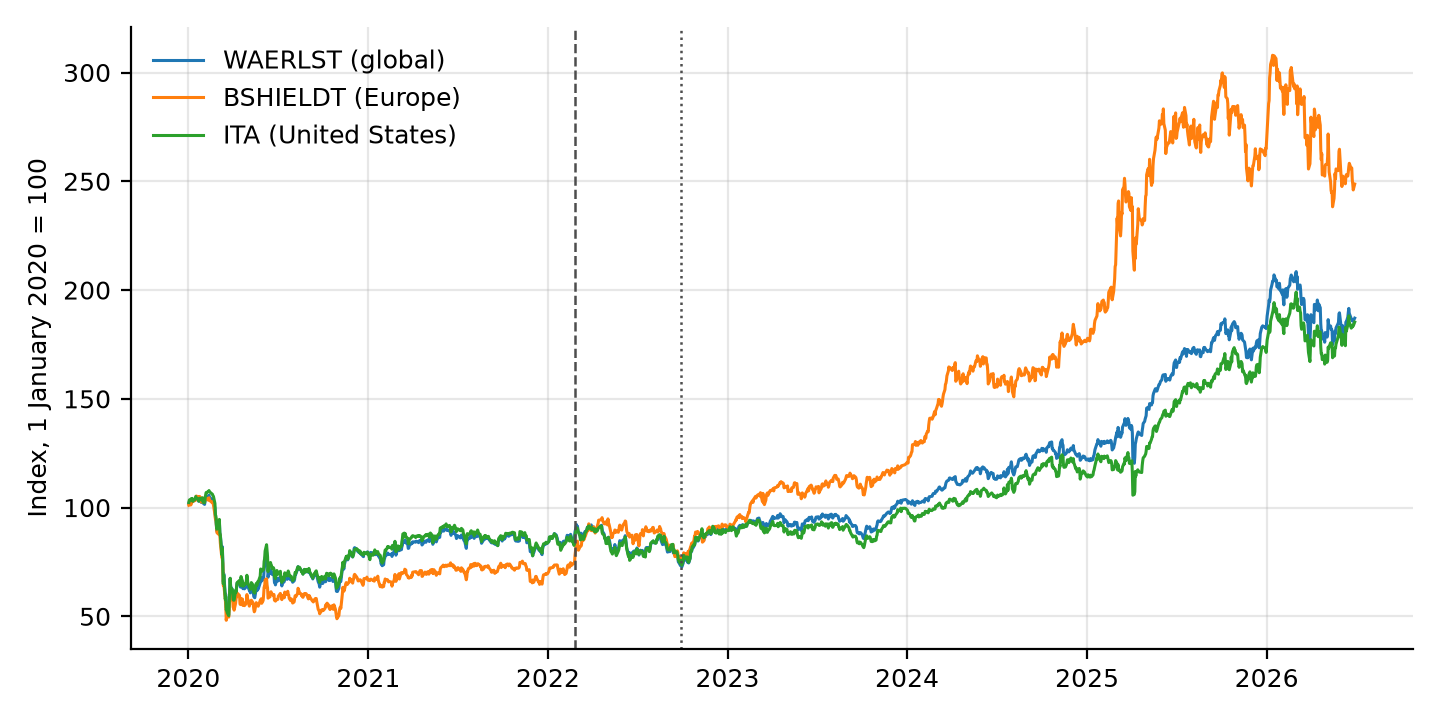
\includegraphics[width=0.78\linewidth,height=0.50\textheight,keepaspectratio]{figures/fig1_defense_indices.png}
\\[0.2em]
{\tiny\color{deckmuted}Defence-equity index levels, 1 January 2020 = 100. Dashed line: 24 February 2022.\par}
\end{center}
\end{frame}
\note{The sharpest repricing of defence equities in decades, in the most intensively covered armed conflict in modern media history. Point at the orange line: two steps, not one -- and the larger of the two is a fiscal announcement rather than battlefield news, which is already a reason to test war news against a market control rather than in isolation.}

\renewcommand{\slidesection}{Why this topic}
\begin{frame}{What the literature establishes --- and the gap}
\footnotesize
\begin{itemize}
\item \textbf{Risk measured from newspaper text.} Baker et al. (2016) and Caldara and Iacoviello (2022) established normalised newspaper counts as a workable proxy. Both are built from a fixed panel of English-language, mostly American and British outlets.
\item \textbf{Media content moves prices.} Tetlock (2007) at short horizons; Manela and Moreira (2017) at long ones.
\item \textbf{Defence equities and conflict are more equivocal than the summaries suggest.} Event studies find sharp responses at onsets --- Covachev and Fazakas (2024) up to 12\%, Klomp (2025) 10--15\%. But continuously measured geopolitical risk predicts defence \emph{volatility}, not returns: Apergis et al. (2018), Zhang et al. (2023).
\item \textbf{The closest paper.} Bondarenko et al. (2024): for the Russian domestic economy, local Russian-language risk measures carry information that English-language measures do not.
\item \textbf{The gap.} No study separates news by the nationality of the outlet that published it. So when a defence-equity price is said to respond to geopolitical risk, it is responding to a quantity built from \textbf{one editorial vantage point} --- and that vantage point is an untested modelling assumption.
\end{itemize}
\end{frame}
\note{The last bullet is the hinge of the whole talk. Say it slowly. Bondarenko is the paper this thesis mirrors: they run the test on the Russian economy, this runs it on the counterparty's assets.}

\renewcommand{\slidesection}{Research question and contribution}
\begin{frame}{Research question and contribution}
\small
\begin{itemize}
\item \textbf{Whose perception of geopolitical risk is priced in defence equities?}
\item Two candidate answers:
\begin{itemize}
\item \emph{Either} the information originates where the war is fought --- local media are closer, cover it earlier and far more heavily --- and reaches Western prices with a delay.
\item \emph{Or} local coverage adds nothing once the Western signal is already in the regression.
\end{itemize}
\item Only the second is directly testable, because it is a statement about \textbf{incremental} information. Establishing the positive claim that Western coverage is itself priced would need a different design, and is not claimed here.
\item \textbf{Contribution.} (i) The mirror of Bondarenko et al. (2024), run on the counterparty's assets. (ii) The editorial vantage point made the object of study rather than an assumption. (iii) A methodological point: at corpus level, this class of measurement error is invisible in the output. (iv) A refinement of the defence-equity literature --- the response is specific to the Western reporting layer.
\end{itemize}
\end{frame}
\note{Be precise about the asymmetry between the two candidate answers. The design identifies an incremental contribution and nothing more; every version of the claim in the thesis is careful about this, and the committee will test whether the talk is too.}

\renewcommand{\slidesection}{Data sources and sample}
\begin{frame}{The measurement problem that dictates the data}
\small
\begin{itemize}
\item Comparing national media ecosystems requires a corpus that actually contains them. The stream most readily available for this --- GDELT's Global Knowledge Graph 1.0 --- does not.
\item A representative daily file holds \textbf{60,690 records}. Of these, \textbf{7} carry a .ru domain and \textbf{21} a .ua domain.
\item Nationality in that stream can be assigned only from the countries an article \emph{mentions}, which for \textbf{88.6\%} of articles is not the country that published it.
\item A series built that way and labelled Ukrainian sentiment therefore measures the tone of \textbf{English-language writing about Ukraine} --- one editorial population sorted by topic and relabelled as three perspectives. Any comparison between them compares two topic proxies, not two vantage points.
\item \textbf{The fix:} GDELT's translingual archive --- \textbf{65 source languages}, machine-translated through a single annotation pipeline, with each article identified by \textbf{the outlet that published it}.
\end{itemize}
\end{frame}
\note{This slide justifies the whole data effort, and it is also contribution (iii): the error is invisible in the output. The series are well behaved, they correlate with events, they differ from one another -- and they are still measuring the wrong thing.}

\renewcommand{\slidesection}{Data sources and sample}
\begin{frame}{Five ecosystems, classified by publisher}
\footnotesize
\begin{itemize}
\item \textbf{UA, RU\_STATE, RU\_INDEP, WEST, EN\_GLOBAL.} An article in a British newspaper about Russian troop movements is Western, not Russian.
\item Four tiers in priority order: a hand-curated register, then national domain suffix, then source language conditional on country, then a residual category.
\item \textbf{Country beats language at every tier.} Ukrainian outlets publish heavily in Russian --- 24tv.ua carries 2,595 Ukrainian-language and 1,865 Russian-language articles. A language-first rule would file those as Russian and manufacture agreement between two ecosystems the design must keep apart.
\item \textbf{One rule, pointing both ways.} State-funded external broadcasters classify to the funding state, which puts Deutsche Welle and RFE/RL in the Western block; exile newsrooms classify to their country of origin, which keeps Meduza in the Russian independent one.
\item \textbf{Validated externally, not asserted.} Each registered domain is resolved against Wikidata: of 84 outlets, 66 resolve and \textbf{63 agree --- precision 0.955}. All three disagreements are exile newsrooms, the one case where origin and operation genuinely differ.
\end{itemize}
\end{frame}
\note{If asked what the audit does not do: it validates that a registered domain belongs to the country assigned to it. It does not validate GDELT's attribution of a given article to a domain -- that would need a reader with Russian and Ukrainian.}

\renewcommand{\slidesection}{Data sources and sample}
\begin{frame}{Variables, targets and sample}
\footnotesize
\begin{itemize}
\item \textbf{Two perception indices per ecosystem per day.} \emph{Ukraine/Russia coverage share} --- articles whose GDELT location field names a place in Ukraine or Russia, over the ecosystem's \textbf{entire} daily output. \emph{Coverage tone} --- mean GDELT tone of those same articles.
\item \textbf{A third, theme-based split} following Caldara and Iacoviello (2022): anticipatory coverage of threats and build-ups against realised coverage of acts and attacks. Conflict-specific by construction.
\item \textbf{Shares, never raw counts.} GDELT source coverage drifts by a factor of two and a half over eleven years; a count series would show that drift as a trend in every ecosystem at once.
\item \textbf{Changes, never levels.} In levels every series carries a common war-regime trend that the financial controls already capture.
\item \textbf{Five targets:} Bloomberg WAERLST (global) and BSHIELDT (Europe) from 2020; the ITA ETF back to 2015; and two hand-built equal-weighted baskets.
\item \textbf{Sample: 4,027 days, 18 February 2015 to 20 May 2026, 98\% of calendar days}; 3,073 carry all five ecosystem series. Supplementary: Ukrainian Air Force records --- 3,812 attack records, 102,396 weapons launched, \textbf{74.3\%} intercepted.
\end{itemize}
\end{frame}
\note{Flag the honest limitation now rather than being asked. For a Western outlet, naming a Ukrainian place implies conflict coverage; for a Ukrainian outlet it implies very little, because domestic politics, business and sport all name Ukrainian places. The local series sit near a ceiling. It returns on the conclusions slide, bounded two ways.}

\renewcommand{\slidesection}{Identification strategy and model}
\begin{frame}{Identification strategy and model}
\footnotesize
\begin{itemize}
\item $r_{i,t} = \alpha + \beta_{West} X^{West}_{t} + \beta_{Local} X^{Local}_{t} + \gamma Z_{t} + \varepsilon_{i,t}$
\item The object of interest is a \textbf{joint }\textbf{$F$}\textbf{-test on }\textbf{$\beta_{Local}$}\textbf{, with the Western block already in the regression.} That conditioning is what separates local media adding something from local and Western media correlating with returns for the same reason.
\item \textbf{The positive control is the identical test on }\textbf{$\beta_{West}$}\textbf{, in the same cells.} If the design detects neither block, a null on the local block means nothing. This is what makes the result a finding.
\item \textbf{The market control must be regional.} European defence returns are controlled with the STOXX 600, not the S\&P 500. Over the build-up the two markets correlate only 0.409, so a US control leaves ordinary European variation in the residual --- and that residual correlates 0.26 with the threat measure being tested.
\item Two controls only, plus HAC(5) standard errors throughout. The grid crosses two frequencies, six episode windows plus the full sample, and five targets: 70 cells, of which \textbf{31} clear a minimum-observation rule.
\item \textbf{31 tests at 5\% would produce about 1.5 false rejections by chance}, so Benjamini--Hochberg correction is applied across all 31 at a 5\% false discovery rate. Gates 3, 4 and 5 are \textbf{pre-registered}; \textbf{Gate 2 is not}, and is reported as the exploratory test it is.
\end{itemize}
\end{frame}
\note{Do not blur the pre-registration line: Gate 2 was never pre-registered and the thesis says so explicitly. For Gates 4 and 5 the data were collected only after the pre-registration was committed, so the ordering is verifiable from commit timestamps rather than asserted.}

\renewcommand{\slidesection}{Results}
\begin{frame}{Descriptive: two media worlds, an order of magnitude apart}
\footnotesize
\begin{itemize}
\item Local outlets: \textbf{71--85\%} of output names a Ukrainian or Russian place. Western: \textbf{7.2\%}. Native-English: \textbf{5.4\%}.
\item At the invasion Western attention moves \textbf{19.0\% to 40.9\%} in a day --- Ukrainian only 90.3\% to 95.8\%.
\item \textbf{The local ecosystems had almost no headroom left to react.}
\end{itemize}
\vspace{-0.35em}
\begin{center}

\includegraphics[width=0.78\linewidth,height=0.50\textheight,keepaspectratio]{figures/fig1_attention_full_sample.png}
\\[0.2em]
{\tiny\color{deckmuted}Ukraine/Russia coverage share by ecosystem, 30-day moving averages, 2015--2026.\par}
\end{center}
\end{frame}
\note{The order-of-magnitude gap is sustained across eleven years, and the gap between the upper three lines and the lower two is the whole point of the panel. Native-English moves 11.8\% to 23.8\% on the same two days, Russian state 84.6\% to 91.2\%. This is the mechanical reason a Western investor watching coverage volume would have seen a signal in Western outlets and very little in local ones: a series already at four-fifths of output cannot rise much when the event arrives.}

\renewcommand{\slidesection}{Results}
\begin{frame}{Descriptive: the tone asymmetry at the invasion}
\footnotesize
\begin{itemize}
\item Tone shift at the invasion: Ukrainian \textbf{$-1.66$}, native-English $-0.64$, Western $-0.36$ --- \textbf{Russian state }\textbf{$+0.02$}.
\item \textbf{Not a composition artefact:} on a fixed panel of the 24 state outlets present on both sides, the shift is \textbf{$-0.05$}.
\item \textbf{The signal that moved most sharply at the defining event of the sample is not the one prices track.}
\end{itemize}
\vspace{-0.35em}
\begin{center}

\includegraphics[width=0.72\linewidth,height=0.45\textheight,keepaspectratio]{figures/fig2_tone_full_sample.png}
\\[0.2em]
{\tiny\color{deckmuted}Mean coverage tone by ecosystem, 30-day moving averages, 2015--2026.\par}
\end{center}
\end{frame}
\note{Russian state media's tone did not change when Russia invaded Ukraine, and Russian independent moved +0.09. Several state outlets became more positive -- Gazeta.ru +0.48, Ren.tv +0.43 -- which is what one would expect from outlets covering the launch of an operation their government had announced as a success. A supremum-Wald test for a break at an unknown date puts Ukrainian tone's largest break on 24 February 2022 and Russian state tone's 393 days later. This is the largest and most robust descriptive fact in the corpus. Note it is the state-versus-Ukraine contrast; the state-versus-independent comparison does not survive and is not claimed.}

\renewcommand{\slidesection}{Results}
\begin{frame}{Gates 2 and 3: local perception and defence-equity returns}
\scriptsize
\begin{center}
\scriptsize
\setlength{\tabcolsep}{4pt}
\renewcommand{\arraystretch}{1.12}
\begin{tabularx}{\linewidth}{Lcccc}
\toprule
\textbf{Block and news timing} & \textbf{Cells} & \textbf{BH surv.} & \textbf{Min. $p$} & \textbf{Verdict} \\
\midrule
\multicolumn{5}{@{}l}{\itshape Gate 2 --- coverage volume and tone (exploratory)} \\
Local, lagged one day (primary) & 31 & 1 & $9.0\times10^{-4}$ & not robust \\
Local, same-day & 31 & 7 & $2.2\times10^{-6}$ & not tradeable \\
Western, lagged one day (control) & 31 & 0 & $2.7\times10^{-3}$ & not detected \\
\addlinespace[2pt]
\multicolumn{5}{@{}l}{\itshape Gate 3 --- anticipated/realised split (pre-registered)} \\
Local, lagged one day (primary arm) & 31 & 2 & $5.5\times10^{-6}$ & \textbf{FAIL} \\
Western, lagged one day (control) & 31 & 2 & $1.6\times10^{-4}$ & \textbf{detected} \\
\bottomrule
\end{tabularx}
\end{center}
\vspace{-0.4em}
{\tiny\color{deckmuted}\textit{Notes:} Joint $F$-tests on one block, with the other block and the controls already in the regression. Benjamini--Hochberg at 5\% FDR across all 31 cells of an arm.\par}
\vspace{0.3em}
\begin{itemize}
\item \textbf{The timing contrast is the sensitivity evidence.} Local coverage is detected in \textbf{7 of 31} cells when credited to its publication day, and in \textbf{1 of 31} when lagged one trading day so that all of it precedes the open --- and that one cell is the 2017--19 window on ITA at weekly frequency, years before the full-scale invasion.
\item \textbf{Gate 3 fails both pre-registered arms.} The build-up window produces no survivor (smallest $p$ 0.018), and the two that do survive share a window where the rule required two. Both are weekly cells fitting 13 parameters to 58 observations, while the grid's two deepest cells --- 2,754 observations --- return $p = 0.08$ and 0.36.
\item \textbf{The Western block is detected in the same 31 cells, under the same correction.} That asymmetry is what the test was built to isolate.
\end{itemize}
\end{frame}
\note{If asked what the seven-to-one collapse proves: it is consistent with same-day news being impounded within the trading day, with a mechanical artefact of matching a return to coverage partly published after it, and with information that decays inside 24 hours. Daily aggregates cannot separate those. What it does establish is narrower and enough -- the design detects the local block readily under the permissive alignment, so the null under the conservative one is not a failure to measure.}

\renewcommand{\slidesection}{Results}
\begin{frame}{Gates 4 and 5: gas and escalation}
\scriptsize
\begin{center}
\scriptsize
\setlength{\tabcolsep}{4pt}
\renewcommand{\arraystretch}{1.12}
\begin{tabularx}{\linewidth}{Lccc}
\toprule
\textbf{Gate and window} & \textbf{$n$} & \textbf{$p$ (local)} & \textbf{$p$ (Western)} \\
\midrule
\multicolumn{4}{@{}l}{\itshape Gate 4 --- Dutch TTF natural gas returns} \\
(a) Build-up and invasion, daily & 222 & 0.399 & \textbf{0.00004} \\
(b) Shutdown and aftermath, daily & 231 & 0.533 & 0.193 \\
(c) Full crisis, daily & 563 & 0.250 & 0.066 \\
(c) Full crisis, weekly & 133 & 0.907 & 0.052 \\
\addlinespace[2pt]
\multicolumn{4}{@{}l}{\itshape Gate 5 --- realised escalation, held-out sample} \\
Horizon $h = 1$ day & 637 & 0.212 & 0.171 \\
Horizon $h = 5$ days & 629 & 0.227 & \textbf{0.033} \\
\bottomrule
\end{tabularx}
\end{center}
\vspace{-0.4em}
{\tiny\color{deckmuted}\textit{Notes:} Both gates were pre-registered before their data were ingested. All four Gate 4 cells estimated are reported.\par}
\vspace{0.3em}
\begin{itemize}
\item These answer the fair objection that \textbf{defence equities are a weak testbed} --- the link from a Russian newspaper to a US contractor's share price runs entirely through Western investors.
\item \textbf{Gas has a direct physical channel:} Russia supplied roughly 40\% of EU gas, and TTF went from about 20 euro to over 300. Yet \textbf{all four pre-registered conditions fail} --- no surviving cell; the Brent placebo breached at $p = 0.0014$; 0.399 becoming 0.840 without the ten largest TTF moves; and the ordering inverted. \textbf{Western detected at }\textbf{$p = 4\times10^{-5}$}\textbf{.}
\item \textbf{Escalation removes prices entirely.} On 637 held-out days local media do not lead realised conflict. The weakest of the four gates: its own Western control is significant at five days, not at one.
\end{itemize}
\end{frame}
\note{The Brent placebo matters because Brent is an asset the supply-signalling mechanism does not predict, so local perception being jointly significant for it is a breach. The inverted ordering is Russian independent rather than Russian state media leading the local block -- the wrong way round for a channel supposed to run through state signalling of supply intent. Gate 4 also shows how a result dissolves under replication alone: estimated on 81 days it returned p = 0.0028, and the pre-registered confirmatory estimate on 222 days of the same calendar period, with nothing altered but the quantity of data, returned 0.399.}

\renewcommand{\slidesection}{Results}
\begin{frame}{Out of sample --- and what a null can bear}
\scriptsize
\begin{center}
\scriptsize
\setlength{\tabcolsep}{4pt}
\renewcommand{\arraystretch}{1.12}
\begin{tabularx}{\linewidth}{Lcc}
\toprule
\textbf{True $R^{2}_{OS}$ implanted} & \textbf{Long sample (1,855 days, 3 targets)} & \textbf{Bloomberg (686 days, 2 targets)} \\
\midrule
0.0\% (nominal size) & 0.02 & 0.02 \\
0.2\% & 0.40 & 0.21 \\
\textbf{0.5\%} & \textbf{0.81} & \textbf{0.44} \\
1.0\% & 0.98 & 0.76 \\
2.0\% & 1.00 & 0.97 \\
\bottomrule
\end{tabularx}
\end{center}
\vspace{-0.4em}
{\tiny\color{deckmuted}\textit{Notes:} Simulated power: rejection rate at the 5\% level, 1,000 paths per cell, so each entry carries a standard error of at most 1.6 percentage points.\par}
\vspace{0.3em}
\begin{itemize}
\item 50 specifications --- five targets by ten predictors --- in an expanding window, one day ahead. Every comparison is \textbf{nested}, so it is arbitrated by \textbf{Clark--West, not Diebold--Mariano}: under nesting DM has no standard normal limiting distribution and is biased against the larger model even when its extra predictor carries real information.
\item \textbf{Zero rejections, against 2.5 expected by chance.} Best $R^{2}_{OS}$ observed \textbf{+0.10\%}; smallest $p$-value 0.067, so not one specification reaches even nominal significance.
\item \textbf{The power simulation is what makes that informative --- and it must be read as two numbers, never one.} On the three long-sample targets an effect of 0.5\% is detected in \textbf{81\%} of paths, and one of 1.0\% in \textbf{98\%}. On the two Bloomberg targets the same effects give \textbf{44\%} and \textbf{76\%}, so there a meaningful effect would be missed more often than not, and the null is weak evidence rather than a bound.
\item \textbf{Power is not exclusion.} 81\% means one sample in five misses a real effect.
\end{itemize}
\end{frame}
\note{The claim is bounded in both directions and must be stated that way: an effect large enough to matter economically would very probably have been seen on the long-sample targets, and an effect that escaped this design lies at or below the bottom of the range the predictability literature treats as economically meaningful. The 0.5 to 1.0\% band is Welch and Goyal (2008) and Campbell and Thompson (2008).}

\renewcommand{\slidesection}{Findings}
\begin{frame}{What this means}
\footnotesize
\begin{itemize}
\item \textbf{Local-language perception adds nothing to defence-equity returns conditional on Western coverage} --- in coverage volume, in tone, in the anticipated/realised structure, across two asset classes, against one non-market outcome, and out of sample. The null is consistent across all four tests.
\item \textbf{This is a finding rather than an absence, because the design demonstrably detects media effects.} The Western block survives correction in the pre-registered anticipation test and is detected at $p = 4\times10^{-5}$ in gas; the local block itself is detected in 7 of 31 cells before the tradeable lag is imposed. The informative feature is the \textbf{co-occurrence} --- a null on the local block in precisely the cells where an effect is found on the Western one.
\item \textbf{The descriptive asymmetry points the same way.} Russian state tone did not move at the invasion and local attention was already at saturation, while Western attention doubled in a day. If the marginal buyers of Western defence equities form their views from Western coverage, they responded to the one series that registered the event.
\item \textbf{The mirror of Bondarenko et al. (2024) comes back reversed --- but the symmetric positive claim is not made.} This design identifies the local block's incremental contribution, not the Western block's own effect. What the two studies jointly support is narrower and more useful: \textbf{the informative ecosystem is the one inhabited by the agents whose decisions are being measured.}
\end{itemize}
\end{frame}
\note{The fourth bullet is where a committee will push. Hold the line: establishing that Western coverage is priced would require it to be detected consistently rather than in some tests and not others, and the evidence falls short of that. Neither result licenses a general claim that local media always or never matter.}

\renewcommand{\slidesection}{Robustness}
\begin{frame}{Robustness: the tests that could have overturned this}
\scriptsize
\begin{itemize}
\item \textbf{The classification rule.} Five rules run through the full grid --- baseline, register-only, no language tier, language-first, and aggregators retained. The verdict is unchanged under all five: one or two survivors of 31. Language-first is the informative failure: it \textbf{cannot represent a Russian independent block at all}, because the language tier claims those articles before ownership is consulted.
\item \textbf{Aggregation.} An index-level null could mask cross-sectional variation. A firm-level panel of \textbf{31 defence names and 85,065 firm-days}, with exposure from published SIPRI arms revenue, produces no exposure gradient in any war window --- nominal significance appears only in the years \emph{before} the full-scale invasion, and \textbf{0 of 10 cells survive correction}.
\item \textbf{The physical war itself}, in case the news measures are simply a poor proxy for it. A forecasting race over \textbf{144 specifications} and five information sets: 16 achieve a positive $R^{2}_{OS}$ and \textbf{none survives correction}. Realised attack intensity is no more informative about subsequent defence returns than perceived intensity.
\item \textbf{Volatility}, where a positive result was most plausible, since volatility is persistent where returns are not. Forty-eight augmented HAR-RV-X specifications: \textbf{none improves significantly}, eight are significantly worse, and all six correction survivors are deteriorations. Reported with its limit --- on a squared-daily-return proxy the HAR family is roughly twice as inaccurate as GARCH, so the test has limited power.
\item Both forecasting exercises are \textbf{exploratory, not pre-registered}, and are labelled that way.
\end{itemize}
\end{frame}
\note{Say plainly that the last two are the weakest evidence in the thesis and that the volatility one is bounded by its own measure. Claiming more for them than they support is exactly the failure the next slide is about.}

\renewcommand{\slidesection}{Robustness}
\begin{frame}{Six results that dissolved --- and why that matters}
\scriptsize
\begin{center}
\scriptsize
\setlength{\tabcolsep}{4pt}
\renewcommand{\arraystretch}{1.12}
\begin{tabularx}{\linewidth}{LL}
\toprule
\textbf{The result, when it was significant} & \textbf{What eliminated it} \\
\midrule
Defence volatility responds to threat & The regional market control (S\&P 500 to STOXX 600) \\
Threat moves returns in the build-up, $p = 0.0001$ & The same control: $p$ becomes 0.84 \\
Gate 3 clears its pre-registered rule, 7 survivors & Adding the held-out window: 7 becomes 2, verdict FAIL \\
Local perception priced in gas, $p = 0.0028$ on 81 days & Replication on 222 days of the same period: $p$ becomes 0.399 \\
Local media anticipate escalation, both halves & The pre-registered held-out sample: $p$ becomes 0.21 \\
A state-versus-independent censorship wedge & Correcting the outlet register: $p = 0.561$ \\
\bottomrule
\end{tabularx}
\end{center}
\vspace{-0.4em}
{\tiny\color{deckmuted}\textit{Notes:} Each correction to the register moved the last one \emph{further} from significance. None of the six is claimed as a result anywhere in the thesis.\par}
\vspace{0.3em}
\begin{itemize}
\item Each was significant at conventional levels, each admitted a plausible economic mechanism, and each survived at least one robustness check before failing another. \textbf{The six failure modes are all different} --- two omitted variables, one truncated sample, one small sample, one in-sample split that did not generalise, one composition change.
\item \textbf{In every case the eliminating test is one that a study reporting the positive would have had no particular reason to run.} That is what bounds how much confidence a single significant specification warrants in this literature.
\item They are reported rather than suppressed because \textbf{in a literature whose regressors are constructed from text, the set of choices under which a result survives is part of the result} --- and a null established against this background is considerably more informative than one obtained without it.
\end{itemize}
\end{frame}
\note{This is the methodological core, and the strongest answer to 'how do we know you did not simply fail to find something'. The honest framing: the project generated six plausible positives and killed all six with tests it chose to run on itself.}

\renewcommand{\slidesection}{Conclusions}
\begin{frame}{Conclusions}
\scriptsize
\begin{itemize}
\item \textbf{The answer.} Local coverage provides no robust incremental information about defence-equity returns beyond what Western coverage already carries. It is a null, not a reversal --- and it is not attributable to a design unable to detect media effects.
\item \textbf{The implication beyond this conflict.} Multilingual geopolitical-risk indicators are built on the premise that sources closer to an event carry information Anglophone coverage omits. Tested in close to the most favourable setting available --- eleven years, the most intensively covered conflict in modern media history, an asset class whose valuation rests on it, local media at near-saturation coverage --- \textbf{the premise does not hold at either horizon at which the information could have been traded.} It is not refuted in general. It cannot be assumed.
\item \textbf{Limitations, stated as bounds.} The coverage-share measure is close to a domestic-news filter for local outlets, so part of the null may be a ceiling --- bounded by Gate 3, which is theme-based and returns the same null, and by local daily changes being two to four times as variable as Western ones. The design is associational, not causal. GDELT tone is dictionary-based. And daily aggregates cannot resolve intraday timing; only timestamped data could settle what the Gate 2 contrast means.
\item \textbf{Extensions.} Other conflicts --- Israel--Hamas, the Taiwan Strait --- to separate a general property of defence-equity pricing from a feature of this war. Intraday prices, at which the anticipated-versus-realised distinction becomes observable. And assets whose marginal investors are \textbf{not} Western, which is the sharpest available test of the proposition that each market prices the information ecosystem its own participants inhabit.
\end{itemize}
\end{frame}
\note{Close on the last extension: it is the proposition the whole thesis converges on, and the one a future paper could actually settle.}

\appendix
\renewcommand{\slidesection}{Backup}
\begin{frame}[plain]
\vspace{2.5em}
{\color{deckaccent}\rule{\linewidth}{2pt}}\par\vspace{1.5em}
{\usebeamerfont{title}\color{deckink}\bfseries Backup slides\par}
\vspace{0.6em}
{\color{deckmuted}Held for questions.\par}
\end{frame}

\renewcommand{\slidesection}{Backup}
\begin{frame}{The main specification, estimated}
\scriptsize
\begin{center}
\tiny
\setlength{\tabcolsep}{4pt}
\renewcommand{\arraystretch}{1.12}
\begin{tabularx}{\linewidth}{Lcccc}
\toprule
 & \textbf{(1) Controls} & \textbf{(2) +Western} & \textbf{(3) +local, same-day} & \textbf{(4) +local, lagged} \\
\midrule
$\Delta$ Ukrainian attention &  &  & 0.009 & $-0.011$ \\
$\Delta$ Russian state attention &  &  & $-0.001$ & $-0.001$ \\
$\Delta$ Russian indep. attention &  &  & $-0.125^{***}$ & 0.010 \\
$\Delta$ Ukrainian tone &  &  & $-0.073^{*}$ & $-0.038$ \\
$\Delta$ Russian state tone &  &  & $0.127^{**}$ & $-0.055$ \\
$\Delta$ Russian indep. tone &  &  & 0.033 & $-0.017$ \\
STOXX 600 return & $0.925^{***}$ & $0.923^{***}$ & $0.927^{***}$ & $0.921^{***}$ \\
Log VIX (lagged) & 0.068 & 0.066 & 0.075 & 0.066 \\
\addlinespace[2pt]
Observations & 921 & 921 & 921 & 921 \\
$R^{2}$ & 0.348 & 0.351 & 0.365 & 0.354 \\
$p$, local block jointly zero & --- & --- & \textbf{0.003} & 0.734 \\
$p$, Western block jointly zero & --- & 0.333 & 0.688 & 0.177 \\
\bottomrule
\end{tabularx}
\end{center}
\vspace{-0.4em}
{\tiny\color{deckmuted}\textit{Notes:} Dependent variable: daily percentage return on BSHIELDT, over the 921 days on which it trades and all five news series exist. News regressors are standardised first differences, so a coefficient is the return change per one-standard-deviation move. Western-block coefficients omitted for space; none is significant. Newey--West HAC(5). Stars: 1\%, 5\%, 10\%.\par}
\vspace{0.3em}
\begin{itemize}
\item Column (3) against column (4) is the whole story in one cell: the local block is jointly significant same-day at \textbf{$p = 0.003$}, and jointly indistinguishable from zero at \textbf{$p = 0.734$} once lagged by one trading day.
\end{itemize}
\end{frame}
\note{Show this if anyone asks to see magnitudes rather than p-values. Regressors are standardised, so a coefficient reads as the percentage-point return change per one-standard-deviation move.}

\renewcommand{\slidesection}{Backup}
\begin{frame}{Does the classification rule drive the result?}
\small
\begin{itemize}
\item Five rules are run through the full 31-cell grid: the \textbf{baseline}; \textbf{register-only}, dropping the ccTLD and language tiers; \textbf{no language tier}; \textbf{language-first}; and one \textbf{retaining news aggregators}.
\item \textbf{The local-block verdict is unchanged under all five} --- one or two survivors of 31 under the primary alignment in every variant.
\item \textbf{Language-first is the informative failure.} Because the language tier claims Russian-language articles before ownership is consulted, it produces \textbf{no Russian independent block at all}. That is the concrete cost of getting the country-before-language rule wrong, and it is why the rule is stated as a rule rather than applied case by case.
\item Three outlets were in fact misfiled under the state-broadcaster rule before it was written down --- which is why that rule is stated in both directions.
\end{itemize}
\end{frame}
\note{Source: outputs/tables/classifier\_sensitivity.csv.}

\renewcommand{\slidesection}{Backup}
\begin{frame}{Why the regional market control is decisive}
\small
\begin{itemize}
\item Controlling European defence returns with the S\&P 500 is superficially reasonable --- the two markets are highly correlated over long horizons.
\item \textbf{Over the build-up window their correlation is only 0.409.} A US control therefore leaves a substantial component of ordinary European market variation in the residual.
\item \textbf{That residual correlates 0.26 with the threat measure being tested}, so the omitted regional factor loads onto the variable of interest.
\item The consequence: a build-up threat effect significant at \textbf{$p = 0.0001$} under the S\&P 500 control becomes \textbf{$p = 0.84$} under the STOXX 600. Two of the six dissolved results share this single cause.
\item Every regression in the thesis therefore uses the regional market return appropriate to its target: STOXX 600 for European targets, S\&P 500 for global and US ones.
\end{itemize}
\end{frame}
\note{If pressed on why this was not obvious from the start: it was not, and that is the point of reporting it. The correlation is high over long horizons and breaks down precisely in the window the test cares about.}

\renewcommand{\slidesection}{Backup}
\begin{frame}{Why Clark--West and not Diebold--Mariano}
\small
\begin{itemize}
\item Forecast-accuracy comparisons in this literature are most often reported with the \textbf{Diebold--Mariano} statistic (1995). It is not valid here.
\item Each of the 50 specifications compares the historical mean \textbf{augmented with one perception predictor} against the historical mean alone. Setting that predictor's coefficient to zero recovers the benchmark exactly, so \textbf{the benchmark is nested within the model}.
\item Under nesting, DM has \textbf{no standard normal limiting distribution} and is \textbf{biased against the larger model} even when its additional predictor carries genuine information --- so a DM-based null here would be partly an artefact of the statistic.
\item \textbf{Clark and West (2007)} correct for the estimation noise that nesting introduces, giving a statistic that is valid in this setting and one-sided in the direction of improvement.
\item Diebold--Mariano with the Harvey et al. (1997) small-sample correction is retained for genuinely non-nested comparisons. In the code the two are separate functions, so the distinction cannot be flagged away.
\end{itemize}
\end{frame}
\note{src/models/evaluation.py keeps them as separate functions deliberately.}

\renewcommand{\slidesection}{Backup}
\begin{frame}{Return forecasting race, by information set}
\scriptsize
\begin{center}
\tiny
\setlength{\tabcolsep}{4pt}
\renewcommand{\arraystretch}{1.12}
\begin{tabularx}{\linewidth}{LLcccc}
\toprule
\textbf{Set} & \textbf{Contents} & \textbf{Specs} & \textbf{$R^{2}_{OS} > 0$} & \textbf{Best $R^{2}_{OS}$} & \textbf{BH surv.} \\
\midrule
F & Financial controls only & 24 & 1 & 0.019 & 0 \\
P & F + physical attack variables & 24 & 4 & 0.073 & 0 \\
N & F + news variables & 24 & 1 & 0.033 & 0 \\
PN & F + physical + news & 24 & 3 & 0.060 & 0 \\
PNG & PN + pairwise ecosystem tone gaps & 24 & 4 & 0.059 & 0 \\
\addlinespace[2pt]
 & Historical mean & 12 & 0 & 0.000 & --- \\
 & AR(1) & 12 & 1 & 0.009 & --- \\
\bottomrule
\end{tabularx}
\end{center}
\vspace{-0.4em}
{\tiny\color{deckmuted}\textit{Notes:} Expanding-window one-step-ahead forecasts on WAERLST, BSHIELDT and ITA, at horizons of one and five days, on the full sample and on the September 2022 to June 2026 attack subsample. Ridge and gradient boosting, 144 rows in total. Exploratory, not pre-registered.\par}
\end{frame}
\note{Adding physical attack data to the financial controls raises the count of positive-R2 cells from one to four, and none of those four is significant. Baselines win 8 of 12 cells.}

\renewcommand{\slidesection}{Backup}
\begin{frame}{Volatility forecasting race, HAR-RV-X against HAR-RV}
\scriptsize
\begin{center}
\tiny
\setlength{\tabcolsep}{4pt}
\renewcommand{\arraystretch}{1.12}
\begin{tabularx}{\linewidth}{Lccccc}
\toprule
\textbf{Model} & \textbf{Specs} & \textbf{Mean QLIKE gain (\%)} & \textbf{Sig. better} & \textbf{Sig. worse} & \textbf{BH surv.} \\
\midrule
HAR-RV-X (N) & 12 & $-4.4$ & 0 & 1 & 0 \\
HAR-RV-X (P) & 12 & $-65.0$ & 0 & 2 & 2 \\
HAR-RV-X (PN) & 12 & $-62.6$ & 0 & 2 & 2 \\
HAR-RV-X (PNG) & 12 & $-64.8$ & 0 & 3 & 2 \\
\bottomrule
\end{tabularx}
\end{center}
\vspace{-0.4em}
{\tiny\color{deckmuted}\textit{Notes:} Mean QLIKE by model class, lower is better: GARCH 0.95, GJR-GARCH 0.96, EGARCH 0.98, \textbf{HAR-RV 1.93}. That last figure is the limitation, not an aside: realised variance here is the sum of squared daily returns, because intraday prices were not available, so the HAR family is roughly twice as inaccurate as the GARCH family it is normally competitive with.\par}
\vspace{0.3em}
\begin{itemize}
\item Augmenting a volatility model with war variables \textbf{degrades} its accuracy on this measure rather than improving it: of 48 specifications none improves significantly, eight are significantly worse, and all six correction survivors are deteriorations.
\item What \textbf{cannot} be concluded is that conflict news carries no information about defence-equity volatility. A test built on squared daily returns has limited power to detect it.
\end{itemize}
\end{frame}
\note{This is the weakest evidence in the thesis and should be presented that way. Apergis et al. (2018) find geopolitical risk predicting volatility in-sample, which is compatible with this: the question here is out-of-sample accuracy against models that already exploit the persistence of realised variance.}

\renewcommand{\slidesection}{Backup}
\begin{frame}{Does the index-level null hide a cross-section?}
\small
\begin{itemize}
\item The objection is fair: an index-level null could mask cross-sectional variation, with heavily war-exposed firms responding where a diversified index does not.
\item \textbf{A firm-level panel of 31 defence names and 85,065 firm-days}, with exposure measured from published SIPRI arms-revenue data, tests it directly.
\item \textbf{No exposure gradient appears in any war window.} Nominal significance appears only in the years before the full-scale invasion, and in a full sample of which 59\% falls in those years.
\item \textbf{0 of 10 cells survive Benjamini--Hochberg correction.} The index-level result is therefore not an artefact of aggregation.
\item Firm-level constituent and SIPRI exposure data could not be extended further, which is why the thesis carries no cross-sectional chapter and says so.
\end{itemize}
\end{frame}
\note{Source: outputs/tables/exposure\_gradient\_bh.csv.}



\end{document}
